\section{结果与讨论}

\subsection{物相组成与相变行为}

图\ref{fig:xrd}给出同一系列样品（第六组）在 200—900 $^\circ$C 热处理后的 XRD 图谱。200 $^\circ$C 样品在 25$^\circ$ 附近仅有一个宽化的包峰，半高宽达 1.19$^\circ$，其余位置没有可分辨的衍射峰，说明该温度下产物仍以非晶或极细的纳米晶形式存在，热处理尚未提供足够的晶化能。300 $^\circ$C 起图谱中出现明确的锐钛矿衍射峰，峰位与 PDF 卡片（锐钛矿 JCPDS 21-1272、金红石 JCPDS 21-1276）对应的 (101)、(004)、(200)、(105)、(211) 等晶面一致，峰形随温度升高而显著锐化，表明晶化程度与晶粒尺寸同步提高。

\begin{figure}[htbp]
  \centering
  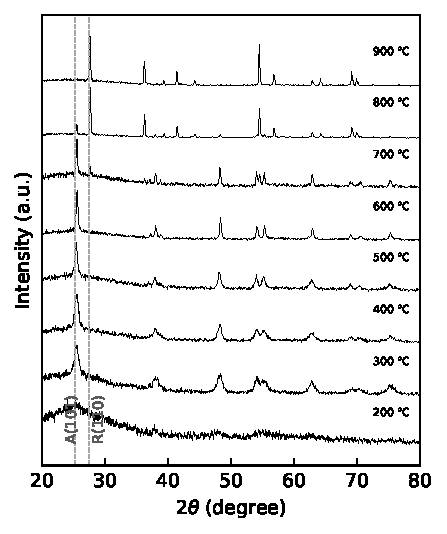
\includegraphics[width=\linewidth]{figures/fig2_xrd_stack.pdf}
  \caption{不同热处理温度下 TiO$_2$ 样品的 XRD 图谱（第六组，2$\theta$=20$^\circ$—80$^\circ$）。虚线分别标出锐钛矿 A(101) 与金红石 R(110) 的标准峰位}
  \label{fig:xrd}
\end{figure}

700 $^\circ$C 时在 27.4$^\circ$ 处出现金红石 (110) 衍射峰，同时 25.3$^\circ$ 的锐钛矿峰仍然存在，说明此时处于两相共存阶段；800 $^\circ$C 时金红石峰成为最强峰，锐钛矿峰明显减弱；900 $^\circ$C 时锐钛矿峰完全消失。各温度下观察到的主要峰位及其归属列于表\ref{tab:peaks}。

\begin{table}[htbp]
  \centering
  \caption{各温度样品主要衍射峰的归属（PDF 标准值对比）}
  \label{tab:peaks}
  \footnotesize
  \begin{tabular}{@{}cccc@{}}
    \toprule
    $2\theta_{\mathrm{obs}}/(^\circ)$ & $2\theta_{\mathrm{PDF}}/(^\circ)$ & $(hkl)$ & 物相 \\
    \midrule
    25.4—25.6 & 25.28 & (101) & 锐钛矿 \\
    37.8      & 37.80 & (004) & 锐钛矿 \\
    48.0      & 48.05 & (200) & 锐钛矿 \\
    54.0      & 53.89 & (105) & 锐钛矿 \\
    55.1      & 55.06 & (211) & 锐钛矿 \\
    27.5      & 27.45 & (110) & 金红石 \\
    36.2      & 36.09 & (101) & 金红石 \\
    41.2      & 41.23 & (111) & 金红石 \\
    54.3      & 54.32 & (211) & 金红石 \\
    56.6      & 56.64 & (220) & 金红石 \\
    \bottomrule
  \end{tabular}
\end{table}

值得指出的是，本文拟合得到的锐钛矿 (101) 峰位在 25.45$^\circ$—25.56$^\circ$ 之间，系统性地高于标准值 25.28$^\circ$ 约 0.2$^\circ$。这一偏差并未随温度单调变化，更可能源于样品表面与样品槽不共面引起的样品位移误差以及仪器零点漂移，而不是晶格畸变，因此在后续定量分析中仅使用同一温度序列内的相对变化。

图\ref{fig:xrdq}与表\ref{tab:xrdq}给出了峰宽、晶粒尺寸与金红石含量的定量结果。晶粒尺寸由 200 $^\circ$C 的 6.8 nm 单调增至 800 $^\circ$C 的 44.8 nm，增长曲线呈现明显的两段特征：300—500 $^\circ$C 区间增长缓慢（9.9→16.9 nm），500—800 $^\circ$C 区间增长加快（16.9→44.8 nm）。这种“先慢后快”的行为说明低温阶段晶粒长大受限于表面扩散与晶界迁移的动力学势垒，而温度超过约 500 $^\circ$C 后热激活使晶界迁移速率显著提高。金红石含量在 200—600 $^\circ$C 始终保持为零，700 $^\circ$C 突增至 17.3\%，800 $^\circ$C 达到 84.7\%，900 $^\circ$C 为 100\%，呈典型的 S 形转变特征，符合“成核—长大”型相变规律：只有当锐钛矿晶粒长大到某一临界尺寸、金红石晶核能够稳定存在时，相变才会迅速推进\cite{zhang2000phase}。

\begin{figure}[htbp]
  \centering
  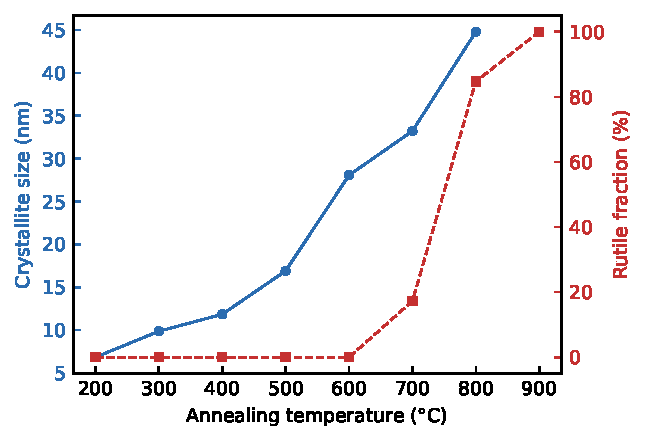
\includegraphics[width=\linewidth]{figures/fig3_xrd_quant.pdf}
  \caption{锐钛矿 (101) 峰对应的 Scherrer 晶粒尺寸与金红石质量分数随热处理温度的变化}
  \label{fig:xrdq}
\end{figure}

\begin{table}[htbp]
  \centering
  \caption{不同热处理温度下的半高宽、晶粒尺寸与金红石含量}
  \label{tab:xrdq}
  \footnotesize
  \begin{tabular}{@{}cccc@{}}
    \toprule
    $T/^\circ$C & FWHM$(101)/(^\circ)$ & $D$/nm & $X_{\mathrm{R}}$/\% \\
    \midrule
    200 & 1.19 & 6.8  & 0 \\
    300 & 0.83 & 9.9  & 0 \\
    400 & 0.69 & 11.8 & 0 \\
    500 & 0.48 & 16.9 & 0 \\
    600 & 0.29 & 28.1 & 0 \\
    700 & 0.25 & 33.2 & 17.3 \\
    800 & 0.18 & 44.8 & 84.7 \\
    900 & ---  & ---  & 100.0 \\
    \bottomrule
  \end{tabular}
\end{table}

为检验结果的可靠性，本文把四个小组在相同温度下的数据做了横向比较（图\ref{fig:groups}）。四组的晶粒尺寸随温度的变化趋势基本重合，在 700 $^\circ$C 均落在 33—41 nm 区间；金红石含量的变化也大体一致。个别数据点偏离趋势：某一小组 800 $^\circ$C 样品未检出金红石且晶粒尺寸偏小（18.4 nm），另一小组 200 $^\circ$C 样品的晶粒尺寸偏大（13.6 nm）。考虑到四组使用的是同一批前驱体与同一台仪器，这类偏离更可能来自装样高度不一致、样品量差异或粉末压实程度不同造成的峰形变化，而非真实的物相差异。这提示在定量比较时，应尽量保证样品制备与装样条件的一致性。

\begin{figure*}[htbp]
  \centering
  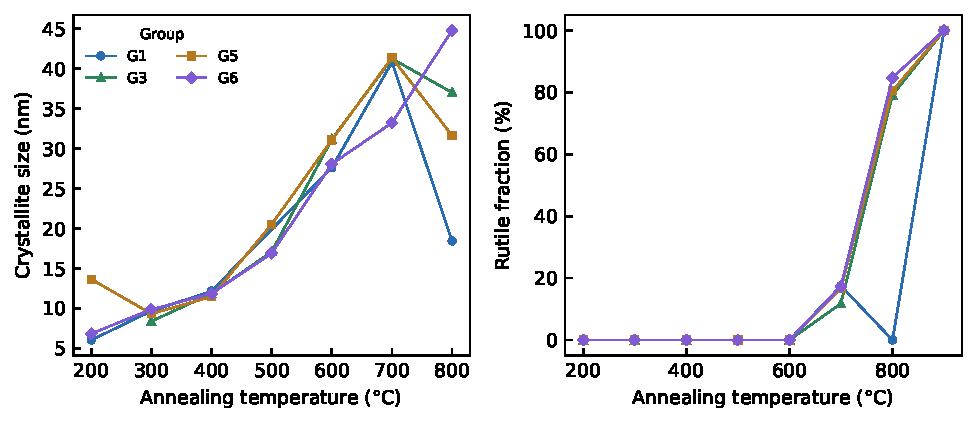
\includegraphics[width=0.74\textwidth]{figures/fig4_xrd_groups.pdf}
  \caption{四个小组数据的重复性比较：(a) 晶粒尺寸；(b) 金红石质量分数随温度的变化}
  \label{fig:groups}
\end{figure*}

\subsection{拉曼光谱对局域结构的验证}

XRD 给出的是长程平均结构信息，而拉曼光谱对短程有序与局域成键更敏感。图\ref{fig:raman}为不同温度样品的拉曼谱（已扣除荧光背景并按 144 cm$^{-1}$ 峰归一化）。400、500、600 $^\circ$C 样品在 144、396—399、515—517 和 639—642 cm$^{-1}$ 处出现清晰谱峰，与锐钛矿的 $E_g$、$B_{1g}$、$A_{1g}+B_{1g}$ 和 $E_g$ 振动模式一一对应；其中 144 cm$^{-1}$ 峰强度最大、随温度升高半高宽逐渐变窄，说明 TiO$_6$ 八面体骨架的短程有序度不断提高，与 XRD 中峰形锐化的结论互相印证。

\begin{figure*}[htbp]
  \centering
  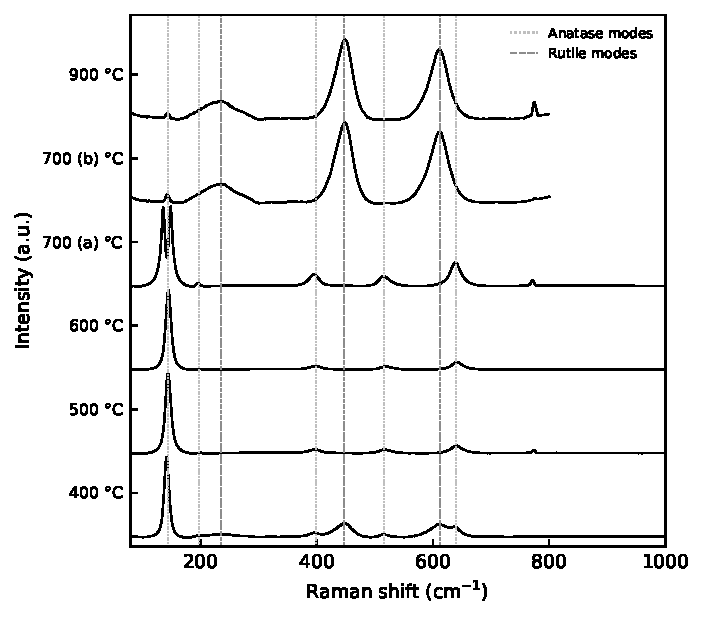
\includegraphics[width=0.56\textwidth]{figures/fig5_raman.pdf}
  \caption{不同热处理温度下 TiO$_2$ 的拉曼光谱（633 nm 激发，已作基线校正与归一化）。点线为锐钛矿特征模式位置，虚线为金红石特征模式位置；700 $^\circ$C 的两个平行样品分别记为 (a) 与 (b)}
  \label{fig:raman}
\end{figure*}

700 $^\circ$C 的两个平行样品呈现出截然不同的谱形：样品 (a) 仍以 149 cm$^{-1}$ 的锐钛矿峰为主，同时 395、515、639 cm$^{-1}$ 峰依然清晰；样品 (b) 则在 143、233、448 和 611 cm$^{-1}$ 处出现金红石的特征峰，其中 448 cm$^{-1}$（$E_g$）与 611 cm$^{-1}$（$A_{1g}$）强度最高。900 $^\circ$C 样品的谱形与样品 (b) 一致，锐钛矿峰完全消失。XRD 给出的 700 $^\circ$C 平均金红石含量为 17.3\%，而拉曼在微米级光斑内却分别观察到“纯锐钛矿”和“纯金红石”两种状态，说明相变在微区尺度上分布极不均匀——这可能与炉内温度梯度、样品堆积厚度导致的局部热历史差异有关。这也解释了为何不同小组在 700 $^\circ$C 附近给出的相含量数据分散度最大。

\begin{table}[htbp]
  \centering
  \caption{拉曼特征峰位及其振动模式归属}
  \label{tab:raman}
  \footnotesize
  \setlength{\tabcolsep}{3pt}
  \begin{tabular}{@{}lccc@{}}
    \toprule
    物相 & 文献/cm$^{-1}$ & 观测/cm$^{-1}$ & 振动模式 \\
    \midrule
    锐钛矿 & 144 & 142—149 & $E_g$ \\
           & 197 & 197     & $E_g$ \\
           & 399 & 395—399 & $B_{1g}$ \\
           & 516 & 515—517 & $A_{1g}+B_{1g}$ \\
           & 639 & 639—642 & $E_g$ \\
    金红石 & 233 & 233     & 多声子过程 \\
           & 447 & 448     & $E_g$ \\
           & 612 & 610—611 & $A_{1g}$ \\
    \bottomrule
  \end{tabular}
\end{table}

\subsection{形貌演化与粒径统计}

图\ref{fig:sem}给出五个温度点的 SEM 形貌像。200 $^\circ$C 样品表面致密平整，除少量碎屑外看不到可分辨的颗粒，这与 XRD 中宽化包峰所反映的非晶/极细晶状态一致；300 $^\circ$C 时表面出现密集的细小颗粒，边界模糊，平均尺寸约 31 nm；500 $^\circ$C 时颗粒轮廓清晰、尺寸分布较窄，平均 39 nm；700 $^\circ$C 时颗粒明显长大并出现棱角分明的多面体外形，平均 85 nm；900 $^\circ$C 时晶粒已粗化至亚微米尺度，部分区域出现明显的烧结颈与孔洞，说明此时颗粒间已发生显著的固相烧结。

\begin{figure*}[htbp]
  \centering
  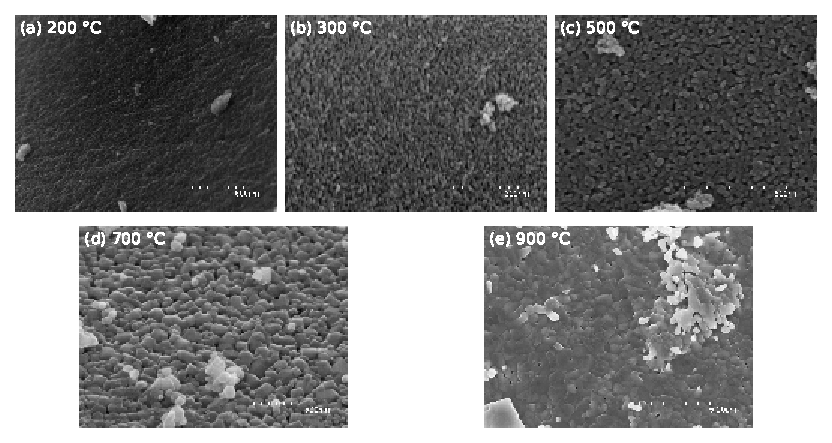
\includegraphics[width=0.74\textwidth]{figures/fig6_sem.pdf}
  \caption{不同热处理温度下 TiO$_2$ 样品的 SEM 形貌：(a) 200 $^\circ$C；(b) 300 $^\circ$C；(c) 500 $^\circ$C；(d) 700 $^\circ$C；(e) 900 $^\circ$C（图中标尺为仪器原始标尺）}
  \label{fig:sem}
\end{figure*}

图\ref{fig:hist}为 300、500、700 $^\circ$C 样品的粒径分布直方图，统计结果汇总于表\ref{tab:size}。三个温度下的分布均近似单峰且略有右偏，标准差随温度升高而增大（11→28 nm），说明高温下颗粒生长的随机性增强。将 SEM 统计的颗粒尺寸与 XRD 的晶粒尺寸比较可以发现，两者相差约 1.5—2.5 倍：500 $^\circ$C 时颗粒 39 nm 而晶粒 16.9 nm，700 $^\circ$C 时颗粒 85 nm 而晶粒 33.2 nm。这一差异说明 SEM 观察到的“颗粒”多为若干一次晶粒构成的聚集体，颗粒内部仍存在晶界；同时也提醒在用不同方法表征“尺寸”时必须明确所指的物理量。

\begin{figure*}[htbp]
  \centering
  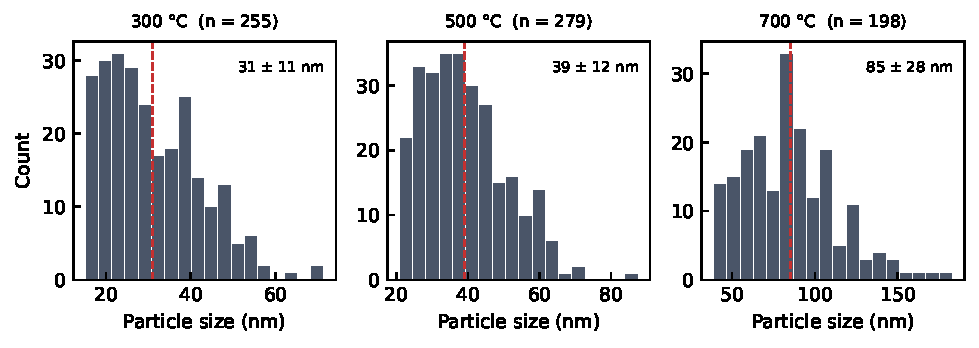
\includegraphics[width=0.72\textwidth]{figures/fig7_sem_hist.pdf}
  \caption{300、500、700 $^\circ$C 样品的粒径分布（虚线为平均值）}
  \label{fig:hist}
\end{figure*}

\begin{table}[htbp]
  \centering
  \caption{SEM 粒径统计结果}
  \label{tab:size}
  \footnotesize
  \setlength{\tabcolsep}{2.4pt}
  \begin{tabular}{@{}ccccc@{}}
    \toprule
    $T/^\circ$C & nm/px & $N$ & $d$/nm & 中位数/nm \\
    \midrule
    200 & 2.83 & --- & 无明显颗粒 & --- \\
    300 & 1.32 & 255 & 31$\pm$11 & 28 \\
    500 & 1.80 & 279 & 39$\pm$12 & 37 \\
    700 & 2.83 & 198 & 85$\pm$28 & 83 \\
    900 & 18.04 & 64 & 942$\pm$622 & 743 \\
    \bottomrule
  \end{tabular}
\end{table}

作为对照，静电纺丝产物的形貌与上述颗粒体系完全不同。纺丝得到的是一层连续的无纺纤维膜，纤维直径中位数约 0.48 $\mu$m（由骨架距离变换统计，$n\approx2.7\times10^{4}$ 个采样点，均值 0.61 $\mu$m、标准差 0.41 $\mu$m），纤维之间存在大量交叉搭接，从而形成高孔隙率的网络结构；同时可观察到直径数微米的珠状缺陷（beads），这是射流在飞行过程中表面张力占优、未能充分拉伸所致，与表\ref{tab:es}中关于浓度、电压与推进速率的分析一致。纤维形貌使该路线产物在比表面积与回收便利性上优于粉体，但在相同热处理条件下其相组成仍由温度决定。

\subsection{能谱分析}

图\ref{fig:eds}为 500 与 900 $^\circ$C 样品的 EDS 谱。两张谱中均只出现 C $K\alpha$（0.28 keV）、O $K\alpha$（0.53 keV）、Ti $L\alpha$（0.45 keV）、Ti $K\alpha$（4.51 keV）与 Ti $K\beta$（4.93 keV）等特征峰，未检出其他金属杂质；1.49 keV 处的弱峰对应 Al $K\alpha$，来自承载样品的铝基底或样品台。C 信号强度随温度升高而下降，与高温下有机残留被充分烧除、表面吸附碳减少的规律一致。需要说明的是，受样品表面粗糙度与计数率限制，本次测试只做了定性成分确认，未进行定量归一化，因此不宜据此讨论 Ti/O 原子比。

\begin{figure}[htbp]
  \centering
  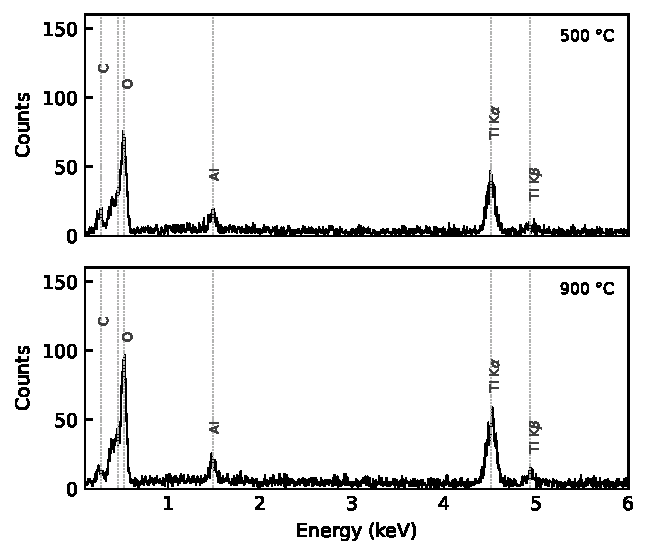
\includegraphics[width=\linewidth]{figures/fig8_eds.pdf}
  \caption{500 $^\circ$C 与 900 $^\circ$C 样品的 EDS 谱（10 kV）}
  \label{fig:eds}
\end{figure}

\subsection{光学性质与带隙}

图\ref{fig:uv}为 400—800 $^\circ$C 样品的紫外-可见吸收谱。所有样品在 400 nm 以下均表现出强吸收，吸收边随热处理温度升高逐渐向长波方向移动：400—600 $^\circ$C 样品的吸收边约在 390 nm，700 $^\circ$C 移至约 400 nm，800 $^\circ$C 进一步红移至约 415 nm。这一红移与金红石相的出现及晶粒长大相对应，因为金红石的带隙（约 3.0 eV）小于锐钛矿（约 3.2 eV），且晶粒增大使量子尺寸效应减弱\cite{serpone1995size}。

\begin{figure}[htbp]
  \centering
  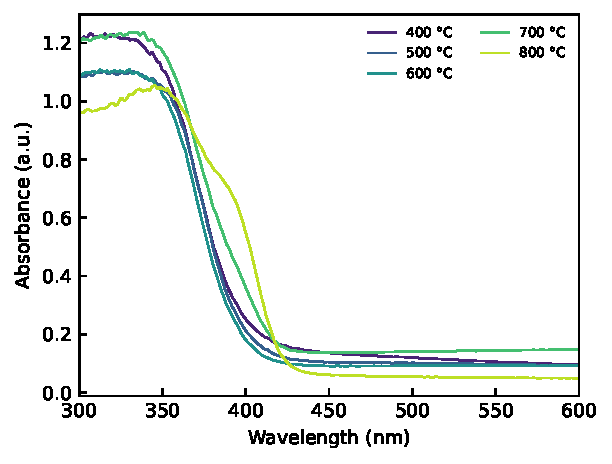
\includegraphics[width=\linewidth]{figures/fig9_uvvis.pdf}
  \caption{不同热处理温度下 TiO$_2$ 的紫外-可见吸收光谱}
  \label{fig:uv}
\end{figure}

将吸收谱按式\eqref{eq:km}与式\eqref{eq:tauc}转换为 Tauc 曲线（图\ref{fig:tauc}），对吸收边线性段作切线外推，得到各样品的表观带隙（表\ref{tab:eg}）：400、500、600 $^\circ$C 分别为 3.12、3.12、3.13 eV，与锐钛矿的文献值 3.2 eV 接近而略低，可能与纳米颗粒表面态及氧空位引起的带尾吸收有关；700 $^\circ$C 降至 3.05 eV，800 $^\circ$C 进一步降至 2.80 eV，与金红石含量由 17.3\% 增至 84.7\% 的趋势一致。800 $^\circ$C 样品的 Tauc 曲线在 3.0 eV 附近存在明显的肩部，线性区判定对 Eg 的影响可达 $\pm0.05$ eV，因此该数值应视为上限估计。

\begin{figure}[htbp]
  \centering
  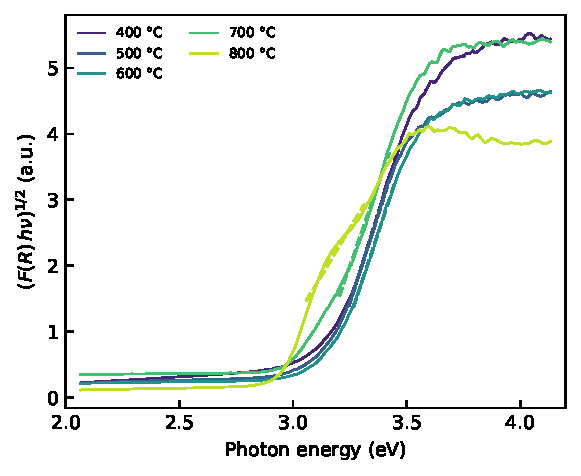
\includegraphics[width=\linewidth]{figures/fig10_tauc.pdf}
  \caption{由 Kubelka-Munk 函数转换得到的 Tauc 曲线及线性外推（虚线）}
  \label{fig:tauc}
\end{figure}

\begin{table}[htbp]
  \centering
  \caption{各温度样品的表观禁带宽度}
  \label{tab:eg}
  \footnotesize
  \begin{tabular}{@{}cccc@{}}
    \toprule
    $T/^\circ$C & 主要物相 & $X_{\mathrm{R}}$/\% & $E_g$/eV \\
    \midrule
    400 & 锐钛矿 & 0    & 3.12 \\
    500 & 锐钛矿 & 0    & 3.12 \\
    600 & 锐钛矿 & 0    & 3.13 \\
    700 & 锐钛矿+金红石 & 17.3 & 3.05 \\
    800 & 金红石为主 & 84.7 & 2.80 \\
    \bottomrule
  \end{tabular}
\end{table}

需要说明的是，900 $^\circ$C 样品的吸收谱基线未正确归零（吸光度出现负值），数据不可靠，故未纳入带隙分析。这一细节也提示在漫反射测试中，参比白板的清洁度与基线扫描步骤对结果影响很大。

\subsection{综合讨论}

把四类表征结果放在同一温度坐标下，可以得到一条自洽的演化链条：200 $^\circ$C 时前驱体尚未完成晶化，产物近于非晶；300—600 $^\circ$C 区间锐钛矿晶粒由 10 nm 长到 28 nm，颗粒由 31 nm 长到 39 nm，禁带宽度稳定在 3.12—3.13 eV；700 $^\circ$C 是相变的临界区间，金红石开始成核并快速长大，微区上锐钛矿与金红石并存，宏观带隙下降；800—900 $^\circ$C 金红石成为主相甚至唯一相，晶粒与颗粒同时粗化至亚微米级，带隙进一步红移。相变温度（600—700 $^\circ$C）与溶胶-凝胶法 TiO$_2$ 的文献报道一致\cite{zhang2000phase,chen2007tio2}，说明本文的热处理制度是合理的。

制备路线的作用主要体现在宏观组装形态上：溶胶-凝胶法得到的是颗粒堆积体，颗粒之间以点接触为主，比表面积大但回收困难；静电纺丝法得到的是连续纤维膜，纤维直径约 0.5 $\mu$m，长径比高、易于分离回收，但存在珠状缺陷。两者在相同温度下的相变行为并无本质差异，说明决定相组成的仍是热处理历史而非成型方式。若面向光催化应用，可考虑利用纤维膜的可回收性，并通过控制煅烧温度在锐钛矿/金红石混合相区间（约 700 $^\circ$C）获得有利于电荷分离的界面结构\cite{ohtani1997mixture}。

本文的分析仍存在若干不足。其一，Scherrer 公式未扣除仪器宽化与晶格应变，所得晶粒尺寸为表观下限值，对于 200 $^\circ$C 这类峰形严重宽化的样品误差更大；其二，金红石含量采用直接对比法，只使用了一对衍射峰，未做 Rietveld 全谱精修，绝对误差估计为 $\pm5\%$；其三，SEM 粒径统计依赖半自动分割，对粘连颗粒存在过分割或漏分割，人工核查估计相对误差约 10\%—15\%；其四，漫反射谱只测量了 300—600 nm，未覆盖近红外区，Tauc 外推的线性区选择带有主观性。后续若能补充 Rietveld 精修、BET 比表面积与 TEM 观察，将能更准确地描述“晶粒—颗粒—团聚体”的多级结构。




